\section{Saturated consolidation}

Equation system (\ref{eqn:pu_eqn}) is solved with a one-step monolithic algorithm.
Moreover, the Newton-Raphson method is adopted to deal with  the nonlinearity.

\subsection {Poro-elastic column (1D)}
%%%%%%%%%%%%%%%
\subsubsection*{Problem definition}
The  example  is a simple one dimensional problem for which an analytical formula for its
solution is known. We consider a porous column bounded by rigid and
impermeable walls, except on its top where a mechanical pressure
load $\sigma_0$ is prescribed and which is free to drain. Suppose
that the length of the column is $H$.
The boundary and initial
conditions for the problem are depicted in Figure \ref{fig:column}:
\begin{figure}[!htb]
\centering
\begin{picture}(250,200)

\put(90,160){\line(1,0){30}} \put(120,10){\line(0,1){150}}
\put(90,160){\line(0,-1){150}}

%\multiput(70,10)(0,11){14}{\line(0,1){7}}

\put(95,185){\vector(0,-1){25}} \put(100,185){\vector(0,-1){25}}
\put(105,185){\vector(0,-1){25}} \put(110,185){\vector(0,-1){25}}
\put(115,185){\vector(0,-1){25}}

\put(80,155){\vector(0,-1){25}}

\linethickness{2pt} \put(90,10){\line(1,0){30}}

%labels
\put(50,160){$x=0$} \put(50,8){$x=H$}
% BC
\put(130,160){$p=0$ , $\sigma=\sigma_0$} \put(130,10){$\partial
p/\partial x=0$ , $u=0$}
% IC
%\put(130,85){$p=0$ , $\partial u/\partial x=0$}
\end{picture}
\caption{Column test problem} \label{fig:column}
\end{figure}
The analytical solution for this problem can be found in
\cite{MurLou:92} as
\begin{eqnarray}
\sigma_D
&=&
-1
+ \sum_{n=0}^{\infty} \frac{2}{M} \sin(M x_D)\,\mbox{e}^{-M^2 t_D}
\nonumber
\\
u_D
&=&
1 - x_D
-
\sum_{n=0}^{\infty}
\frac{2}{M} \cos(M x_D)\, \mbox{e}^{-M^2 t_D}
\\
\Pressure_D
&=&
\sum_{n=0}^{\infty}
\frac{2}{M} \sin(M x_D)\,\mbox{e}^{-M^2 t_D}
\nonumber
\end{eqnarray}
%
where $x_D=x/H$, $t_D=(\lambda+2\mu)kt/\eta H^2$, $M=1/2
\pi(2n+1)$ are non-dimensional quantities and
$\sigma_D=\sigma/\Pressure_0$, $u_D=u(\lambda+2\mu)/\Pressure_0
H$, $\Pressure_D=\Pressure/\Pressure_0$ are dimensionless
effective stress, displacement and pore pressure, respectively.
\subsubsection*{Material properties}
The material
parameters used in the computation are given in Table
\ref{ex1_TableHM1}. The load put on the strip is $-10^3$Pa, time step
size is $\Delta t=1.0$s and the total simulation time is $t=10$s.

\begin{table}[h]
\centering
  \begin{tabular}{lll}
   \hline \hline
    Parameter & Unit & Value \\
   \hline
     Young's modulus & $3\times 10^{4}$  & $N/m^{2}$ \\
     Poisson's ratio & $0.2$             & $-$ \\
     Permeability    & $10^{-10}$        & $m^2$ \\
     Fluid viscosity & $10^{-3}$         & $Pa\,s$ \\
   \hline \hline
  \end{tabular}
  \caption{\label{ex1_TableHM1}Material parameters}
\end{table}
\subsubsection*{Results}
Time step size is proposed as $1$s.
Comparison of the results for fluid pressure and effective stress
obtained by the LS-MFEM, GFEM and the analytical solution are shown
in Figure \ref{ex1_fig1}
\begin{figure}[!htb]
  \begin{center}
  \epsfig{figure=HM/cregp010.eps,height=5cm}
  \epsfig{figure=HM/cregs010.eps,height=5cm}

  \epsfig{figure=HM/cregp210.eps,height=5cm}
  \epsfig{figure=HM/cregs210.eps,height=5cm}

  \epsfig{figure=HM/cregp410.eps,height=5cm}
  \epsfig{figure=HM/cregs410.eps,height=5cm}
  \end{center}
  \caption{Simulated fluid pressures (left) and effective stress (right)
  at time $t$=10s by grids from the coarsest to finest one}
  \label{ex1_fig1}
\end{figure}

\subsubsection*{Benchmark deposit}
\begin{tabular}{|l|l|l|}
  \hline
  Benchmark & Problem type & Path in benchmark deposit \\
  \hline
 \emph{hm\_tri}& HM & benchmarks\verb \HM\ \\
  \hline
\end{tabular}
%%%%%%%%%%%%%%%%%
%%%%
\subsection {Poro-elastic cube (3D)}
\label{sec:hm_foot}
\subsubsection*{Problem definition}
We consider a vertical cross-section through a
homogeneous soil. Due to symmetry we can limit the investigation
to half of the domain. The model domain is then extending 8 meters
in length and 5 meters in height. The problem is solved  in  2D and 3D space, respectively.
\subsubsection*{Initial and Boundary conditions}
Boundary conditions are: strip
loading ($\sigma_{yy}=\sigma_0$ in $x\in[0,1]$), zero stresses
($\sigma_{yy}=\sigma_{xy}=0$ in $x\in(1,8]$) and zero pressure at
the top; no horizontal flux, no horizontal displacements and zero
shear stresses at left and right hand sides; no vertical flux and
no displacements at bottom (Figure \ref{fig-setting}).
\begin{figure}[!htb]
\begin{picture}(380,190)
\put(70,160){\line(1,0){240}}
\put(310,10){\line(0,1){150}}
\multiput(70,10)(0,11){14}{\line(0,1){7}}
\put(75,180){\vector(0,-1){20}}
\put(80,180){\vector(0,-1){20}}
\put(85,180){\vector(0,-1){20}}
\put(90,180){\vector(0,-1){20}}
\put(95,180){\vector(0,-1){20}}
\put(308,165){8}
\put(60,165){0}
\put(55,8){-5}
% BC
% left
\put(5,100){$\frac{\partial p}{\partial x} = 0$}
\put(5,85) {$u_x = 0$}
\put(5,75) {$\sigma_{xy} = 0$}
% top
\put(75,150){$\sigma_{yy}=\sigma_0$}
\put(75,140){$\sigma_{xy}=0$}
\put(180,165){$\sigma_{xy}=\sigma_{yy}=0$}
\put(210,187){\vector(1,0){100}}
\put(175,187){\vector(-1,0){105}}
\put(180,185){$p=0$}
% right
\put(320,100){$\frac{\partial p}{\partial x} = 0$}
\put(320,85) {$u_x = 0$}
\put(320,75) {$\sigma_{xy} = 0$}
% bottom
\put(160,-5){$\frac{\partial p}{\partial y} = 0$ , $u_x=u_y=0$}
\linethickness{2pt}
\put(70,10){\line(1,0){240}}
\end{picture}
\caption{Footing problem}
\label{fig-setting}
\end{figure}

\subsubsection*{Material properties}
 The material properties of the porous medium for this case are given in Table
\ref{tab:materials_case1}.
\begin{table}[!htb]
\centering
\caption{Material properties}
\label{tab:materials_case1}
%
% For LaTeX tables use
%
\begin{tabular}{lll}
\hline\hline
Property & Value & Unit \\
\hline
Young's modulus & $3\times 10^{4}$  & $N/m^{2}$ \\
Poisson's ratio & $0.2, 0.4$       & $-$ \\
Permeability    & $10^{-10}$        & $m^2$ \\
Fluid viscosity & $10^{-3}$         & $Pa\,s$ \\
\hline \hline
\end{tabular}
\end{table}
\subsubsection*{Results}
 The geometry is to expand the 2D domain
  by extruding the 2D shape of 1m in off-plane direction (\ref{fig_HM3}).
\begin{figure}[!htb]
  \begin{center}
  \epsfig{figure=HM/HM3D/g2d.eps,height=5.5cm}
  \epsfig{figure=HM/HM3D/g3d.eps,height=5cm}
  \end{center}
  \caption{Analyzed models}
  \label{fig_HM3}
\end{figure}
 Results at the critical step, i.e., the first step, are shown in Fig. \ref{fig:e10},  \ref{fig:e11}
 and  \ref{fig:e12}
\begin{figure}[!thb]
  \begin{center}
   %%\vspace{-2.7cm}
   \begin{minipage}[t]{0.45\textwidth}
     \begin{center}
    \includegraphics[scale=0.3]{HM/HM3D/pre.eps}
    \centerline{Pressure [Pa]}
    \end{center}
   \end{minipage}
  %%\hspace{0.01\textwidth}
   \begin{minipage}[t]{0.45\textwidth}
    \begin{center}
    \includegraphics[scale=0.3]{HM/HM3D/stress_yy.eps}\\
    \centerline{Vertical stress [Pa]}
    \end{center}
   \end{minipage}\\
  \end{center}
  \caption{2D: distribution}
  \label{fig:e10}
\end{figure}
%%%
\begin{figure}[!htb]
  \begin{center}
   %%\vspace{-2.7cm}
   \begin{minipage}[t]{0.40\textwidth}
     \begin{center}
    \includegraphics[scale=0.25]{HM/HM3D/pre3d.eps}
    \centerline{Pressure [Pa]}
    \end{center}
   \end{minipage}
  %%\hspace{0.01\textwidth}
   \begin{minipage}[t]{0.4\textwidth}
    \begin{center}
    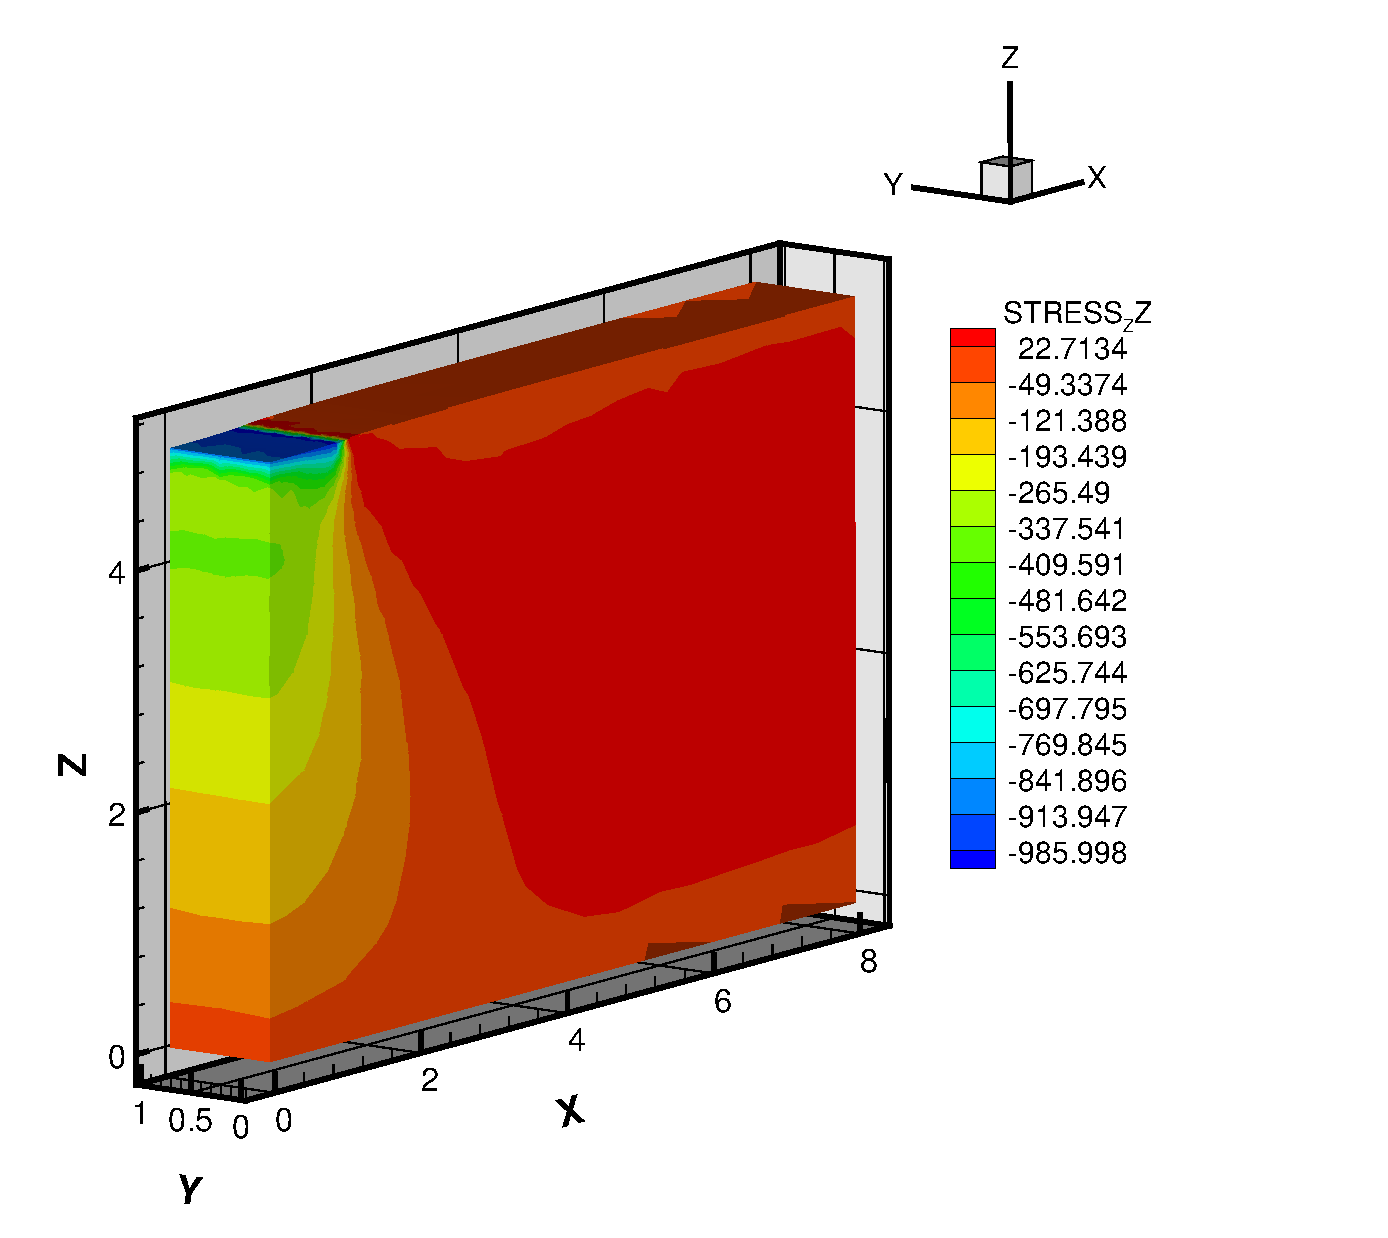
\includegraphics[scale=0.25]{HM/HM3D/stress3d_yy.eps}\\
    \centerline{Vertical stress [Pa]}
    \end{center}
   \end{minipage}\\
  \end{center}
  \caption{3D: distribution}
  \label{fig:e12}
\end{figure}
%%%
\begin{figure}[H]
  \begin{center}
   %%\vspace{-2.7cm}
   \begin{minipage}[t]{0.40\textwidth}
     \begin{center}
    \includegraphics[scale=0.25]{HM/HM3D/pre_line.eps}
    \centerline{Pressure [Pa]}
    \end{center}
   \end{minipage}
  %%\hspace{0.01\textwidth}
   \begin{minipage}[t]{0.4\textwidth}
    \begin{center}
    \includegraphics[scale=0.25]{HM/HM3D/stress_yy_line.eps}\\
    \centerline{Vertical stress [Pa]}
    \end{center}
   \end{minipage}\\
  \end{center}
  \caption{Comparison along symmetrical axis}
  \label{fig:e11}
\end{figure}

The results produced by 2D model with triangle element and 3D model
with tetrahedral element matches each other. This shows that all
objects presented in this study work fine for TH coupling problem.
\subsubsection*{Benchmark deposit}
\begin{tabular}{|l|l|l|}
  \hline
  Benchmark & Problem type & Path in benchmark deposit \\
  \hline
 \emph{hm\_foot\_tri}\&  \emph{hm\_foot\_tet}& HM & benchmarks\verb \HM\ \\
  \hline
\end{tabular}
%%%%%%%%%%%%%%%%%
%%%%

\subsection{Plastic consolidation}
\subsubsection*{Problem definition}
 A quarter of the cylindrical
sample of 5cm in diameter and 10cm in length under constant pressure. We assume that the plastic behavior the sample material
can be represented by the Cam-Clay model and the problem is axisymmetrical.
\subsubsection*{Initial and Boundary conditions}
The initial void ratio $e_0=1.5$ at such initial stress state
\[
\sigma_{r}^0=\sigma_{\theta}^0=\sigma_{z}^0=50kPa
\]
The top of sample is compressed down to 5cm.  While the radial
stress kept constant of $50kPa$, i.e., the traction boundary
condition at cylindrical surface must be zero. Both uncoupled and
coupled cases are analyzed. For the coupled case, drainage is
assigned on the bottom of the sample. The two case should give the
same results. The displacement load is applied in 50 increments.
\subsubsection*{Material properties}
Table \ref{ex3_table1} shows the material parameters.
\begin{table}[htb]
\centering
\label{ex3_table1}
%
% For LaTeX tables use
%
\begin{tabular}{lll}
\hline\hline
Property & Value & Unit \\
\hline
Poisson's ratio & $0.3$       & $-$ \\
Slope of the critical line, M & $1.2$       & $-$ \\
Virgin compression index, $\lambda$ & $0.2$       & $-$ \\
Swelling/recompression index $\kappa$ $0.02$       & $-$ \\
Initial pre-consolidation pressure & $60$       & $kPa$ \\
Permeability    & $10^{-11}$        & $m^2$ \\
Fluid viscosity & $10^{-3}$         & $Pa\,s$ \\
\hline\hline
\end{tabular}
\caption{Material properties}
\end{table}
\subsubsection*{Results}
The evolution of the deviatoric stress along with the axial strain
are demonstrated in Fig. \ref{ex3_q_e}. Both uncoupled (see Section \ref{sec:ccup}) and coupled
cases give the same result as expected\cite{SheSloYu00}.
%Contour plot
\begin{figure}[H]
  \begin{center}
    \includegraphics[scale=0.4]{HM/HM_CC/ex3_c_q_e.eps}\\
  \end{center}
  \caption{ Mises stress vs axial strain: Cam-Clay consolidation}
  \label{ex3_q_e}
\end{figure}
\subsubsection*{Benchmark deposit}
\begin{tabular}{|l|l|l|}
  \hline
  Benchmark & Problem type & Path in benchmark deposit \\
  \hline
\emph{hm\_cc\_tri\_s}& HM & benchmarks\verb \HM\ \\
  \hline
\end{tabular}
%%%%%%%%%%%%%%%%%
\subsection{Dynamic consolidation}
\subsubsection*{Problem definition}
This example is used just to demonstrate that the global assembly of matrices and vectors, the time stepping
 of dynamic problems are dealt with correctly. The example described below is modified from the footing example given
 in Section \ref{sec:hm_foot}.
\subsubsection*{Initial and Boundary conditions}
 All stresses and pressure are zero at the beginning of deformation. Strip
loading ($\sigma_{yy}=\sigma_0$ in $x\in[0,1]$), zero stresses
($\sigma_{yy}=\sigma_{xy}=0$ in $x\in(1,8]$) and zero pressure at
the top; no horizontal flux, no horizontal displacements and zero
shear stresses at left and right hand sides; no vertical flux and no
displacements at bottom (Figure \ref{fig-setting}).
\subsubsection*{Material properties}
Material parameters are given in Table \ref{tab:materials_HMd1}.
\begin{table}[!htb]
\label{tab:materials_HMd1}
\centering
\begin{tabular}{lll}
\hline\hline
{\smallskip}
Property & Value & Unit \\
\hline
Young's modulus & $3\times 10^{4}$  & $N/m^{2}$ \\
Poisson's ratio & $0.2, 0.4$       & $-$ \\
Permeability    & $10^{-10}$        & $m^2$ \\
Fluid viscosity & $10^{-3}$         & $Pa\,s$ \\
\hline\hline
\end{tabular}
\caption{Material properties of dynamic consolidation problem}
\end{table}
\subsubsection*{Results}
Constant time step size of 10s with time damping parameters:
  \[\beta_1=0.51,\,\beta_2=0.515,\,\bar\beta=0.51\]
Time duration is ten time steps.

The following figures, Fig. \ref{fig_dynHM1}--\ref{fig_dynHM4} show the distribution of state variables within the domain after 10 time steps. Such distribution is similar
 to the static case illustrated in Fig. \ref{fig:e10}.
\begin{figure}[!htb]
  \begin{center}
  \epsfig{figure=HM/dyn/pre.eps,height=5cm}
  \epsfig{figure=HM/dyn/pre_rate.eps,height=5cm}
  \end{center}
  \caption{Fluid pressures $p$ and rate of fluid pressure $\dot p$ }
  \label{fig_dynHM1}
\end{figure}
\begin{figure}[!htb]
  \begin{center}
  \epsfig{figure=HM/dyn/ux.eps,height=4cm, width=0.32\textwidth}
  \epsfig{figure=HM/dyn/ux_v.eps,height=4cm, width=0.32\textwidth}
  \epsfig{figure=HM/dyn/ux_a.eps,height=4cm, width=0.32\textwidth}
  \end{center}
  \caption{Displacement, its rate and acceleration: horizontal component}
  \label{fig_dynHM2}
\end{figure}
\begin{figure}[!htb]
  \begin{center}
  \epsfig{figure=HM/dyn/uy.eps,height=4cm, width=0.32\textwidth}
  \epsfig{figure=HM/dyn/uy_v.eps,height=4cm, width=0.32\textwidth}
  \epsfig{figure=HM/dyn/uy_a.eps,height=4cm, width=0.32\textwidth}
  \end{center}
  \caption{Displacement, its rate and acceleration: vertical component}
  \label{fig_dynHM3}
\end{figure}
\begin{figure}[!htb]
  \begin{center}
  \epsfig{figure=HM/dyn/syy.eps,height=6cm, width=0.7\textwidth}
  \end{center}
  \caption{Vertical stress}
  \label{fig_dynHM4}
\end{figure}
\subsubsection*{Benchmark deposit}
\begin{tabular}{|l|l|l|}
  \hline
  Benchmark & Problem type & Path in benchmark deposit \\
  \hline
 \emph{hm\_dyn\_tri}& HM & benchmarks\verb \HM\ \\
  \hline
\end{tabular}
%%%%%%%%%%%%%%%%%
%%%%
